%Deadline Analysis of AUTOSAR OS Periodic Tasks in the Presence of Interrupts: Yanhong Huang et.al
\section{Deadline Analysis of AUTOSAR OS Periodic Tasks in the Presence of Interrupts}

\subsection*{Key Idea}
Provide an abstract framework to determine if the given periodic task will miss its deadline in the presence of interrupts.
Rather than bounding interrupts for given time. Proposes a mechanism to bind the timing calculation to maximum number of interruption allowed to a given task from interrupts.(e.g. The task will meet deadline as long as the number of interrupts is at most n.)
\subsection*{Width and Scope}
Provides a mean to abstract representation of the maximum number of interruption allowed to a task.
Assumptions part of the approach:
\begin{itemize}
	\setlength{\itemsep}{0pt}
	\setlength{\parskip}{0pt}
	\setlength{\parsep}{0pt} 
	\item Tasks are periodic and are implicit in nature with deadline equal to period.
	\item Any task activated by ISR2 will execute and terminate before the end of the ISR.
	\item Resource locking and blocking to the tasks due to it are not considered.
\end{itemize}
Mentions two independent healthiness concept: Task that is not interrupted and tasks that are interrupted.
\begin{figure}[H]
	\centering
	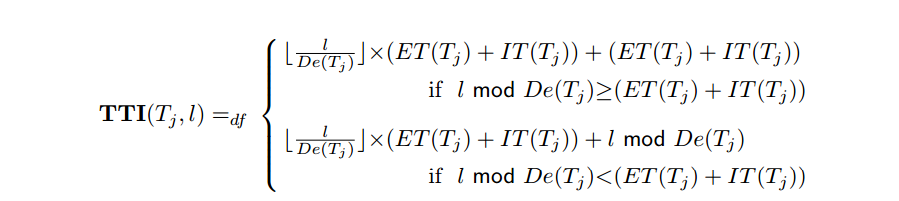
\includegraphics[width=400pt]{Pictures/Autosar_TTI_Bound}
	\caption{Timing Bound formula}\label{abs}
\end{figure}
\subsection*{Experimental Approach}
Experiments done on Mathematica. Total slack available then split to interrupt times.
\subsection*{Conclusion}
Calculate the slack, split it in terms of ISR time.That's main idea.
\subsection*{Link}
http://haslab.uminho.pt/jff/files/2013-deadlineanalysisautosar\_os.pdf